\section{Limiting conditional distribution}



Suppose each individual produces, at the end of its life, independently, a number of offspring that is a random variable $\xx$, with 
$$\pr{\xx = k} = p_k, \hspace{20pt} k = 0,1,2,\dots$$
Denote the mean number of offspring per individual by 
$$\mu=\mean{\xx}$$
Let ${\bf Z}_n$ be the number of individuals in the $n$th generation. Then $\mean{\zz_n|\zz_0=1} = \mu^n.$ If $\mu < 1$ then $\lim_{n\to \infty}{\pr{\zz_n = 0}} = 1$. The population is guaranteed to go extinct.

Denote the probability generating function of $\xx$ as 
$$\phi(z) = \mean{z^{\xx}},$$
and the probability of population extinction by generation $n$ as 
$\pr{\zz_n = 0} = u_n.$
Then, as can be seen from a first step argument, it holds that 
\begin{equation}
\label{iterPGF}
u_{n+1} = \phi(u_n).
\end{equation}

\subsection{Death or division}
Consider the specific case: 
\begin{align*}
p_2 &= P &&\text{(division)}  \\
p_0 &= 1-P && \text{(death)}\\
p_i &= 0 \hspace{20pt} \forall i \neq 0,2  
\end{align*}

\noindent
In this case the mean number of offspring per individual takes the value,
$$\mu = 2P.$$
And so the expected population size resulting from a single offspring will be
$$\mean{\zz_n} = (2P)^n.$$
From (\ref{iterPGF}), we see
\begin{equation}
\label{unIter}
u_{n+1} = 1-P + P u_n^2.
\end{equation}
With $u_n$ the probability of extinction, let us also denote its complement
$$S_n = 1-u_n,$$
the probability of population persistence at generation $n$. 

From (\ref{unIter}), it can be shown that
\begin{equation}
\label{SnIter}
S_{n+1} = 2P S_n - PS_n^2.
\end{equation}

\subsection{Late time persistence probability, $S_n$}

Considering the case where $P < 0.5$, in which death of an individual is more probable than its reproduction, the expected population size will tend towards 0 with increasing $n$; the probability of non-extinction too will approach 0. 

As it does so, $S_n^2$ becomes insignificant in comparison to $S_n$. For this reason, the iterative relation, (\ref{SnIter}), will increasingly satisfy
\begin{equation}
\label{attenuated}
S_{n+1} \approx 2PS_n.
\end{equation}
So at late time ($n\to\infty$), it will be found that
\begin{equation}
\label{lateS}
S_n \sim A\,(2P)^n\qquad (n\to\infty),\quad A=\lim_{m\to\infty}S_m/(2P)^m.
\end{equation}
The multiplying constant, $A$, might be interpreted as those lingering conditions on $S_n$ accumulated before attenuation to (\ref{attenuated}). In any case, it can be demonstrated computationally: 


\begin{figure}[ht]
\centering
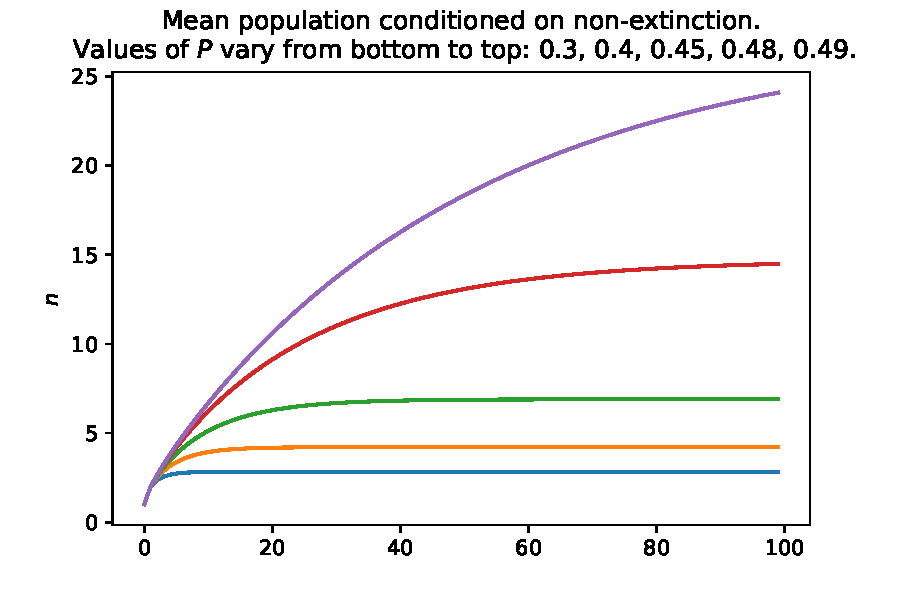
\includegraphics[width = 0.8\textwidth]{figures/IMG_ch3/conditionalMean.pdf}
    \label{fig:image}
\end{figure}

\noindent
Figure \ref{fig:image} shows $(2P)^n / S_n$ plotted over successive generations, $n$. In the code, $S_n$ is calculated iteratively using (\ref{SnIter}). The lines were generated with different values of $P$, those at the top closer to the critical state; the purple line was made with $P = 0.49$, the blue at the bottom, $P=0.3$. It is clear that this ratio will tend to a constant value towards large $n$.  

\subsection{Quasi-stationarity}

It is often the case in stochastic processes, as it is in this one for $P<0.5$, that fixation to a particular state is inevitable. Although, in certain cases, it can be observed that before absorption to some final state, behaviour becomes predictable according to some unchanging distribution. This phenomenon has been termed quasi-stationarity. 


\subsection{Mean}
Such behaviour can be observed in a population evolving by the update rules stated above. For demonstration, consider the mean number of individuals from a single ancestor, conditioned on non-extinction: 
$$\mean{\xx_n} = \pr{\xx_n =0} \cancelto{0}{\mean{\xx_n|\xx_n =0}}  + \pr{\xx_n \neq 0}\mean{\xx_n|\xx_n \neq0}.$$
It follows that 
$$\mean{\xx_n|\xx_n \neq 0} =\frac{\mean{\xx_n}}{\pr{\xx_n\neq 0}} = \frac{(2P)^n}{S_n} .$$ 
Then, due to (\ref{lateS}), as $n\to\infty$
$$\mean{\xx_n|\xx_n \neq 0} \to \frac{(2P)^n}{A(2P)^n} = \frac{1}{A};$$
At late time, the remaining non-extinct population tends to a constant expected size.

\subsection{Variance}

\subsubsection{Computing the second moment, $\mean{\xx_n^2}$}

For a random variable, $\xx$, the moment generating function is defined, $\mean{\ee^{t\xx}}$. It can also be written in terms of the probability generating function, $\phi(\ee^t)$. For variable, $\xx$ in question, the pgf is 
\begin{equation*}
\phi_1(z) = Pz^2 + (1-P),
\end{equation*}
and the mgf is 
\begin{equation}
\label{mgf1}
M_1(t) = \phi_1(\ee^t) = P\ee^{2t} + (1-P).
\end{equation}
The subscript 1 indicates relevance to generation $n = 1$. Moments are obtained from $M_n(t)$ in the following way.
\begin{equation}
\label{mgf2}
\mean{\xx_n^r} = \frac{\dd^r}{\dd t^r} M_n(t)\bigg|_{t=0}.
\end{equation}
For example, to get the second moment of $\xx_1$, we can differentiate (\ref{mgf1}) twice, and evaluate the result at $t=0$:
$$ \frac{\dd^2}{\dd t^2} M_1(t)\bigg|_{t=0} = 4P\ee^{2t}\big|_{t=0} = 4P.$$
Quantifying the process' second moment is important when it comes to computing the population variance for successive iterations. But this is only the second moment of the first generation size. To obtain its value for any generation $n$, we must dig a little deeper.  

Following (\ref{mgf2}), we seek to differentiate the moment generating function twice. To start with, let us represent the $n$th mgf in terms of probability generating functions. Recall,
$$\phi_n(z) = \underset{n \text{ times}}{\underbrace{ \phi_{1}\hspace{-2pt}\lrb{\phi_1\hspace{-2pt}\lrb{\dots\phi_1\hspace{-2pt}\lrb{z}}}    }}.$$  
So it follows that 
$$M_n(t) = \phi_1\lrbq{\phi_1\lrbq{\dots\phi_1\lrbq{\ee^t}}}.$$
Differentiating this once, 
\begin{equation}
\label{dmgf1}
M_n'(t) = \phi_1'\lrbq{\phi_{n-1}\lrbq{\ee^t}}  \cdot  \phi_1'\lrbq{\phi_{n-2}\lrbq{\ee^t}}  \cdots   \phi_1'\lrbq{\phi_{1}\lrbq{\ee^t}} \cdot \phi_1'\lrbq{\ee^t} \cdot\ee^t.
\end{equation}
Because 
$$\phi_1'\lrbq{\phi_k\lrbq{\ee^t}} = \frac{\dd}{\dd \phi_k\lrbq{\ee^t}}\bigg(P[\phi_k\lrbq{\ee^t}]^2 + (1-P)\bigg) = 2P \phi_k\lrbq{\ee^t},$$
and $\phi_1'\lrbq{\ee^t} = 2P\ee^t$, (\ref{dmgf1}) is equivalent to 
$$M_n'(t) = (2P)\phi_{n-1}\lrbq{\ee^t}  \cdot  (2P)\phi_{n-2}\lrbq{\ee^t} \cdots (2P)\phi_{1}\lrbq{\ee^t} \cdot (2P)\ee^{2t}.$$
Which in turn can be written as
\begin{equation}
\label{dmgf2}
M_n'(t) = (2P)^n \cdot M_{n-1}(t)  \cdot  M_{n-2}(t)  \cdots M_{1}(t)  \cdot \ee^{2t}.
\end{equation}
Before differentiating this a second time, it is instructive to note that each of the multiplied components, when evaluated at $t=0$ become 1; $M_k(0) = 1$ $\forall k$, and $\ee^{2\times 0} = 1$. 

So, when evaluating the second derivative at $t=0$, it will be seen that many of the parts simplify. This is because, with the expression being a combination of multiplied functions of $t$, differentiating by $t$ will result in a sum of terms. Each element of the sum will be like (\ref{dmgf2}), but with one of the components differentiated wrt t. This is just the product rule ---
\begin{align*}
M_n''(t) = (2P)^n\bigg[  &M_{n-1}'(t)  \cdot  M_{n-2}(t)  \cdots M_{1}(t)  \cdot \ee^{2t} \\
+ &M_{n-1}(t)  \cdot  M_{n-2}'(t)  \cdots M_{1}(t)  \cdot \ee^{2t} \\
&\hspace{65pt}\cdots\\
+ &M_{n-1}(t)  \cdot  M_{n-2}(t)  \cdots M_{1}'(t)  \cdot \ee^{2t} \\
+ &M_{n-1}(t)  \cdot  M_{n-2}(t)  \cdots M_{1}(t)  \cdot 2\ee^{2t} \bigg].
\end{align*}
And as most of the components become 1 with $t=0$,
\begin{equation*}
M_n''(0) = (2P)^n\lrbs{M_{n-1}'(0) + M_{n-2}'(0) + \cdots + M_1'(0) + 2}.
\end{equation*}
$M_k'(0)$ is simply the mean population at generation $k$, so
\begin{equation*}
M_n''(0) = (2P)^n\lrbs{(2P)^{n-1} + (2P)^{n-2} + \cdots + (2P) + 2} = (2P)^n\lrbs{\sum^{n-1}_{i = 0}\lrb{(2P)^i} + 1}.
\end{equation*}
Using the finite geometric series sum, $\sum_{i=1}^n r^{i-1} = (1-r^n)/(1-r)$, 
\begin{equation*}
\mean{\xx_n^2} = M_n''(0) = (2P)^n\lrbs{\frac{1-(2P)^n}{1-2P} + 1};
\end{equation*}
rearranging,
\begin{equation}
\label{secondMoment}
\mean{\xx_n^2}  = (2P)^n\lrb{1 + \frac{1}{1-2P}} - (2P)^{2n}\lrb{\frac{1}{1-2P}}.
\end{equation}
(The minus sign is required: at $n=1$ the expression must return $\mean{\xx_1^2}=4P$.)



\subsubsection{Late time variance}
Var($\xx_n$) is computed using $\mean{\xx_n^2} - \mean{\xx_n}^2$. With (\ref{secondMoment}), we can write,
$$\text{Var}(\xx_n) = (2P)^n\lrb{1 + \frac{1}{1-2P}} - (2P)^{2n}\lrb{\frac{1}{1-2P}} - (2P)^{2n}.$$
For $2P < 1$, at large $n$, $(2P)^{2n}$ will become insignificant in comparison to $(2P)^n$. Hence, as $n\to\infty$,
$$\text{Var}(\xx_n) \to (2P)^n\lrb{1 + \frac{1}{1-2P}}.$$
It's tempting to jump straight from this, to a conclusion that the variance conditional on $\xx_n \neq 0 $ is stationary. But let's not get ahead of ourselves and start from the conditional moments:
$$\mean{\xx_n^2|\xx_n\neq 0} = \frac{\mean{\xx_n^2}}{S_n} \xrightarrow{n\to\infty}   \frac{(2P)^n\lrb{1 + \frac{1}{1-2P}}}{A(2P)^n} = A^{-1}\lrb{1 + \frac{1}{1-2P}}$$
$$\mean{\xx_n|\xx_n\neq 0} =  \frac{\mean{\xx_n}}{S_n}  \xrightarrow{n\to\infty}    \frac{(2P)^n}{A(2P)^n} = A^{-1}$$
From this, it can be seen that the conditional variance will indeed tend to a constant value at late time:
\begin{equation*}
\text{Var}(\xx_n|\xx_n\neq0) = \frac{1}{A}\lrb{1+\frac{1}{1-2P}} - \frac{1}{A^2}.
\end{equation*}



\subsection{Quantifying the quasi-stationary distribution}

We are yet to compute the constant $A$, but so far, Grant has shown that (\ref{SnIter}) can be written as 
$$S_{n+1} - S_n = -rS_n - PS_n^2,$$
($r = 1-2P$). Which in the large $n$ limit will satisfy
$$\frac{\dd S(x)}{\dd x} = -(1-2P)S_n = PS^2,$$
a Riccati equation with solution
$$S(x) = \frac{rB}{e^{rx} +- PB},$$
$B$ constant. 



%%%%%%%%%%%%%%%%%%%%%%%%%%%%%%%%%%%%%%%%%%%%%%%%%%%%%%%%%%%%%%%%%%%%% special 2 small
